%\documentclass[aps,prd,nofootinbib]{revtex4-1}
\documentclass[singlepage,notitlepage,nofootinbib,11pt]{revtex4-1}
\usepackage{amsmath}
\usepackage{graphicx}
\usepackage{subfig}
\usepackage{epsfig}
\usepackage{listings}
\usepackage[hidelinks,hyperfootnotes=false,bookmarks=false,colorlinks=true]{hyperref}

\newcommand{\eq}[1]{\begin{align*}#1\end{align*}}
\newcommand{\pmat}[1]{\begin{pmatrix}#1\end{pmatrix}}
\newcommand{\center}[1]{\begin{center}#1\end{center}}
\def\<{\langle}
\def\>{\rangle}
\def\l{\left}
\def\r{\right}


\begin{document}
\title{Problem Set 2 - G6080}
\author{Victor Genty}
\email{vgenty@nevis.columbia.edu}
\homepage{www.nevis.columbia.edu/~vgenty}
%\affiliation{Department of Physics, Duke University, Durham, NC 27707, USA}
\date{\today}
\begin{abstract}
\centering
Source code can be found at \href{https://github.com/vgenty/G6080/tree/master/ps3}{github.com/vgenty/G6080/ps3}
\end{abstract}
\maketitle
\section{Problem 1 - Stats of Mock Data}
\begin{center}The code for this problem can be found in \verb|mock_data/mac/one.py|, \verb|mock_data/src/*|, and \verb|mock_data/include/*| \end{center}
\subsection{1.}
The true means for the 5 data sets for all 1,600,000 values are:
\begin{center}
\begin{tabular}{ | c | c | c | c | c |}\hline
  $\overline{v}_1$ &  $\overline{v}_2$ &  $\overline{v}_3$ &  $\overline{v}_4$ &  $\overline{v}_5$  \\ \hline \hline 
  1.76084 & 2.88634 & 4.01185 & 5.13712 & 6.26238 \\ \hline
\end{tabular}
\end{center}
\subsection{2.}
Histograms of sample means are shown in Fig. \ref{histos}. As the number of values in each sample increased, the standard deviation of the means is reduced by a factor of 
\eq{
\delta\sigma\approx\frac{1}{\sqrt{N}}\sim\frac{1}{\sqrt{10}},
}
as expected.
\begin{figure}[h]
  \centering
  \captionsetup[subfigure]{labelformat=empty}
  \subfloat[][]{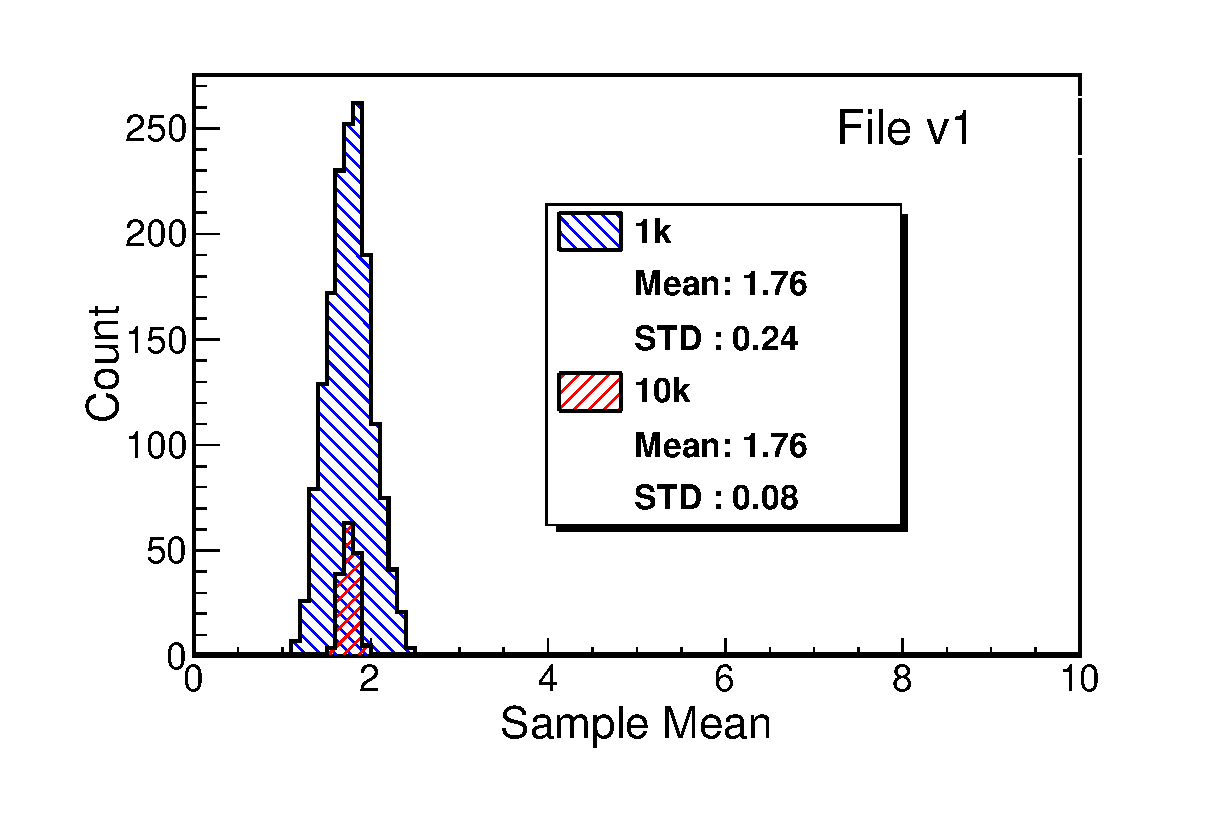
\includegraphics[width=0.5\textwidth]{figures/b1.eps}}
  \subfloat[][]{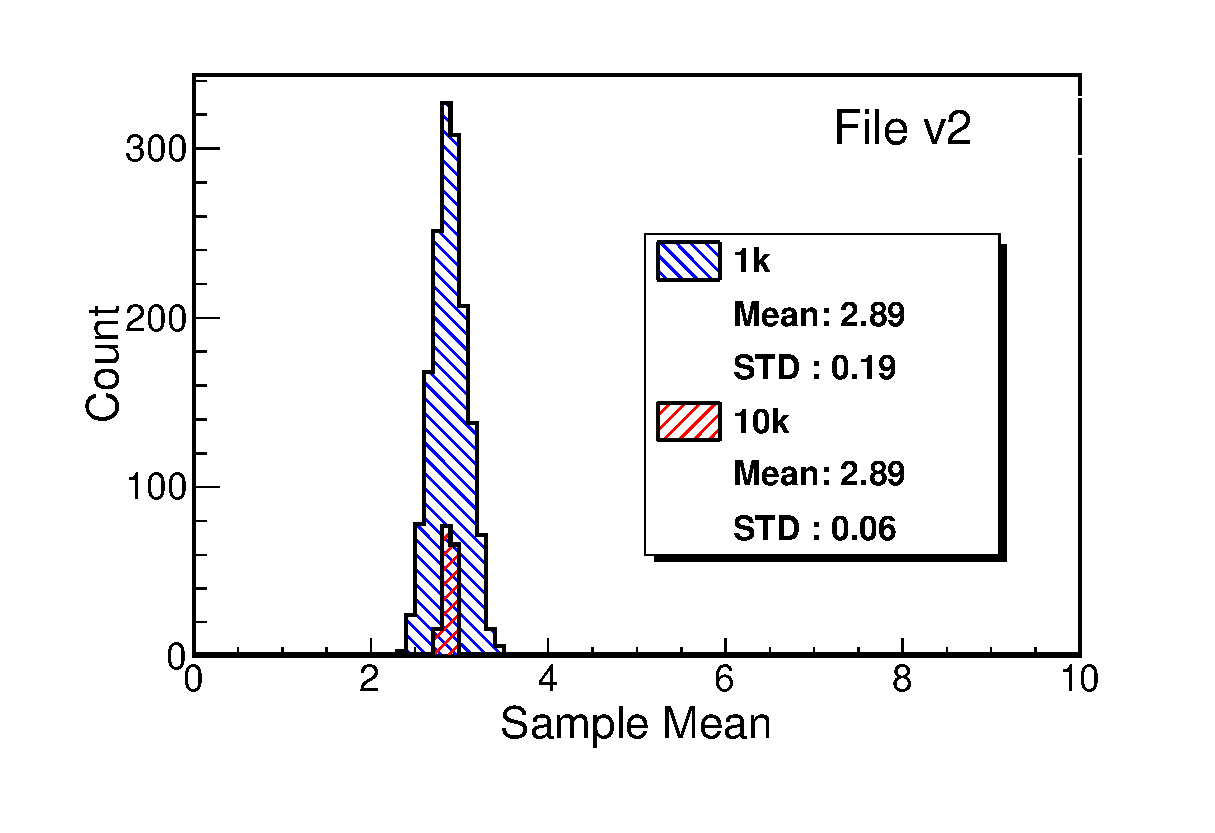
\includegraphics[width=0.5\textwidth]{figures/b2.eps}}\\
  \subfloat[][]{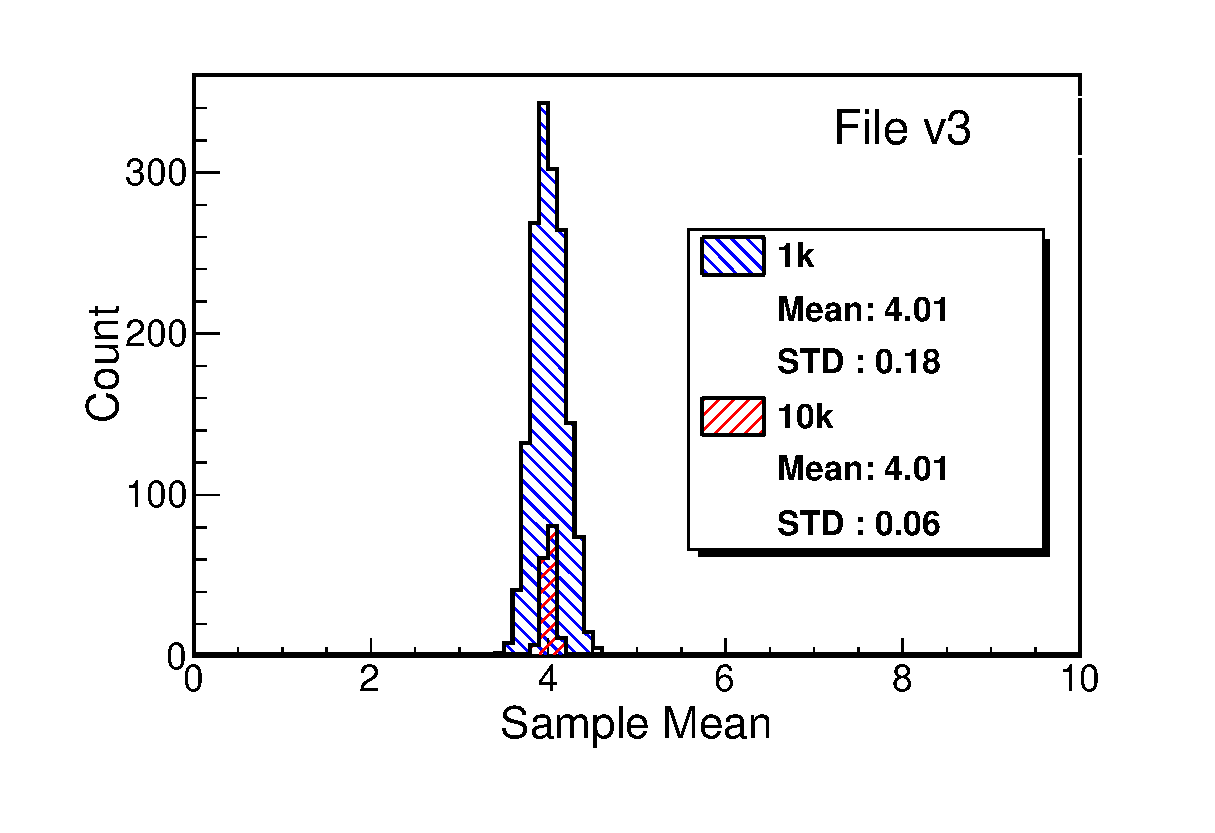
\includegraphics[width=0.5\textwidth]{figures/b3.eps}}
  \subfloat[][]{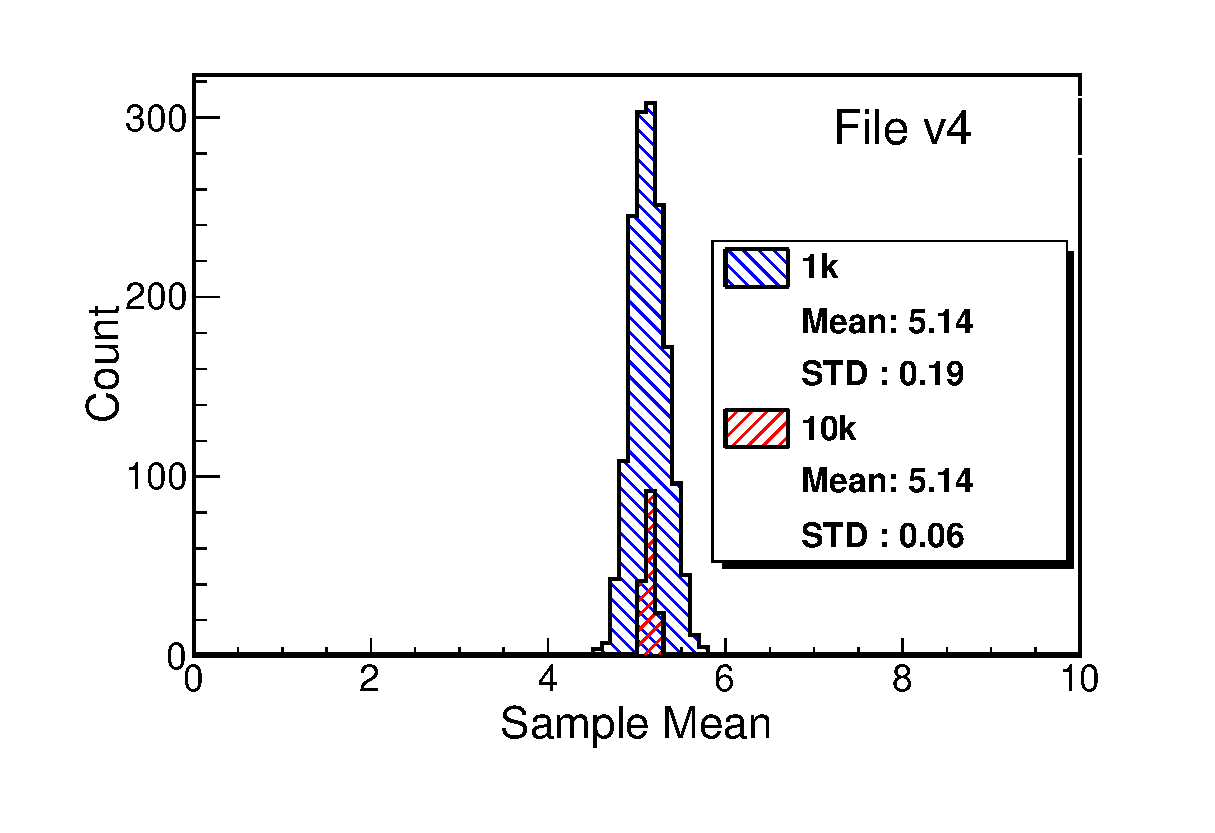
\includegraphics[width=0.5\textwidth]{figures/b4.eps}}\\
  \subfloat[][]{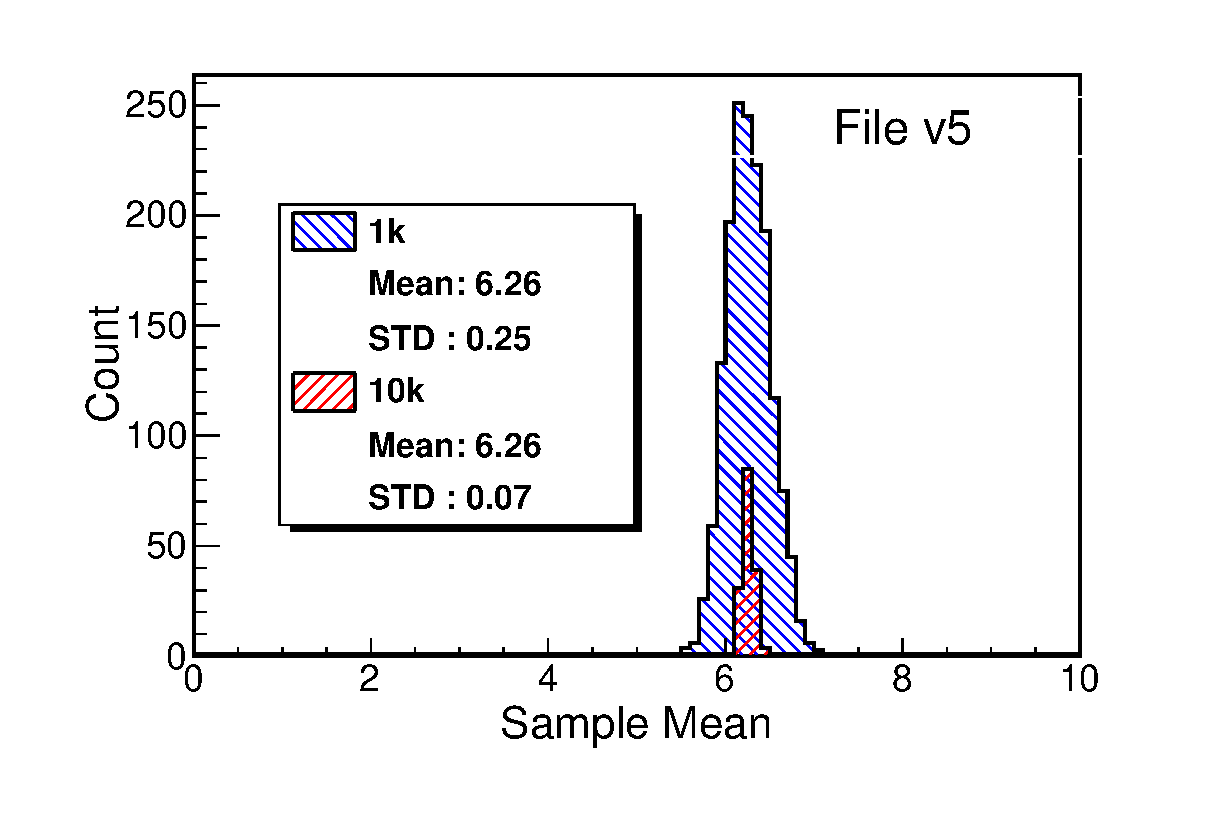
\includegraphics[width=0.5\textwidth]{figures/b5.eps}}
  \caption{\label{histos} Histogram of sample means for 5 data sets. The blue shaded histogram contains the sample means for samples of size 1,000. The red histogram contains the sample means for samples of size 10,000. Increasing the number of sample means in each sample has the expected effect of narrowing the distribution.}
\end{figure}
\clearpage
\subsection{3}
We compute the true autocorrelation function for each of the data sets with the formula given in the problem. The normalized autocorrelation function $C_{v_a}(n)/C_{v_a}(0)$ for each data set is plotted versus $n_{\text{cut}}$ and shown in Fig. \ref{corrs}. The value of $n$ (or $n_{\text{cut}}$) which the auto-correlations disappear is roughly 100.
\begin{figure}[h]
  \centering
  \captionsetup[subfigure]{labelformat=empty}
  \subfloat[][]{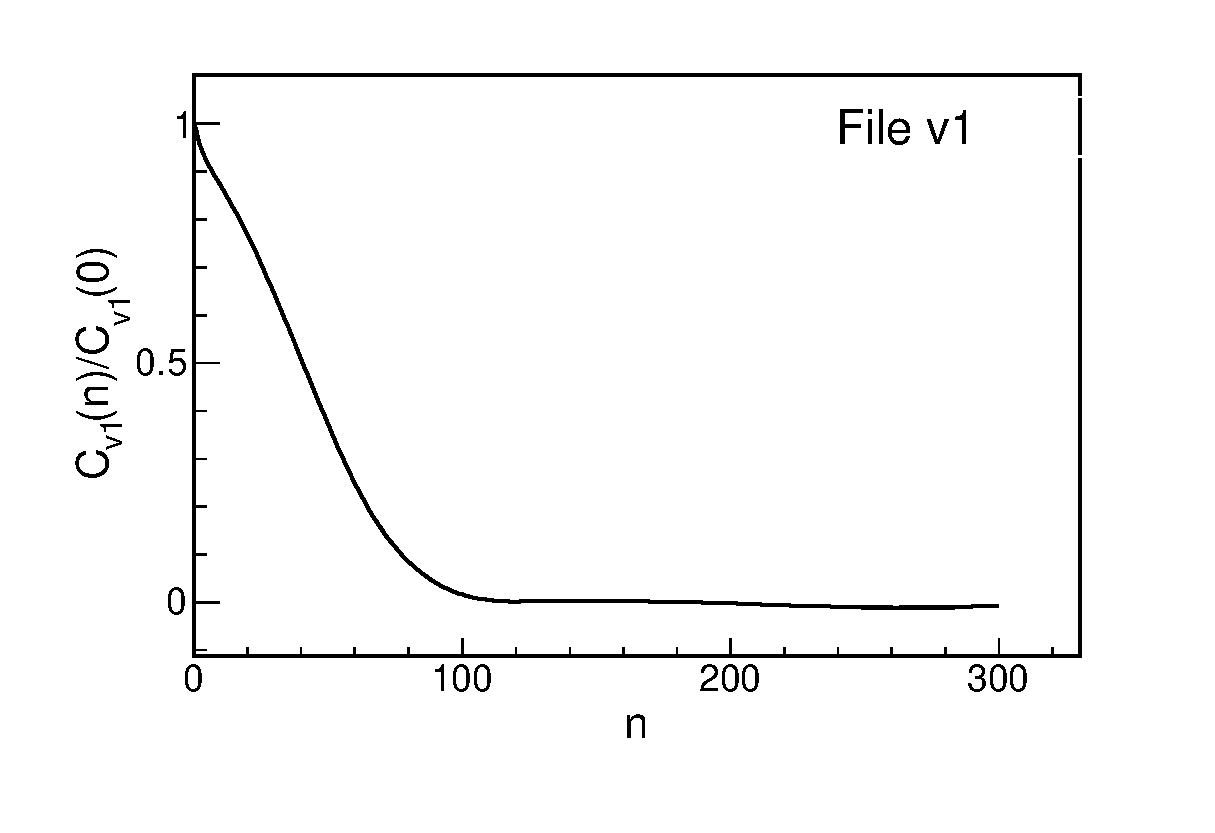
\includegraphics[width=0.5\textwidth]{figures/c1.eps}}
  \subfloat[][]{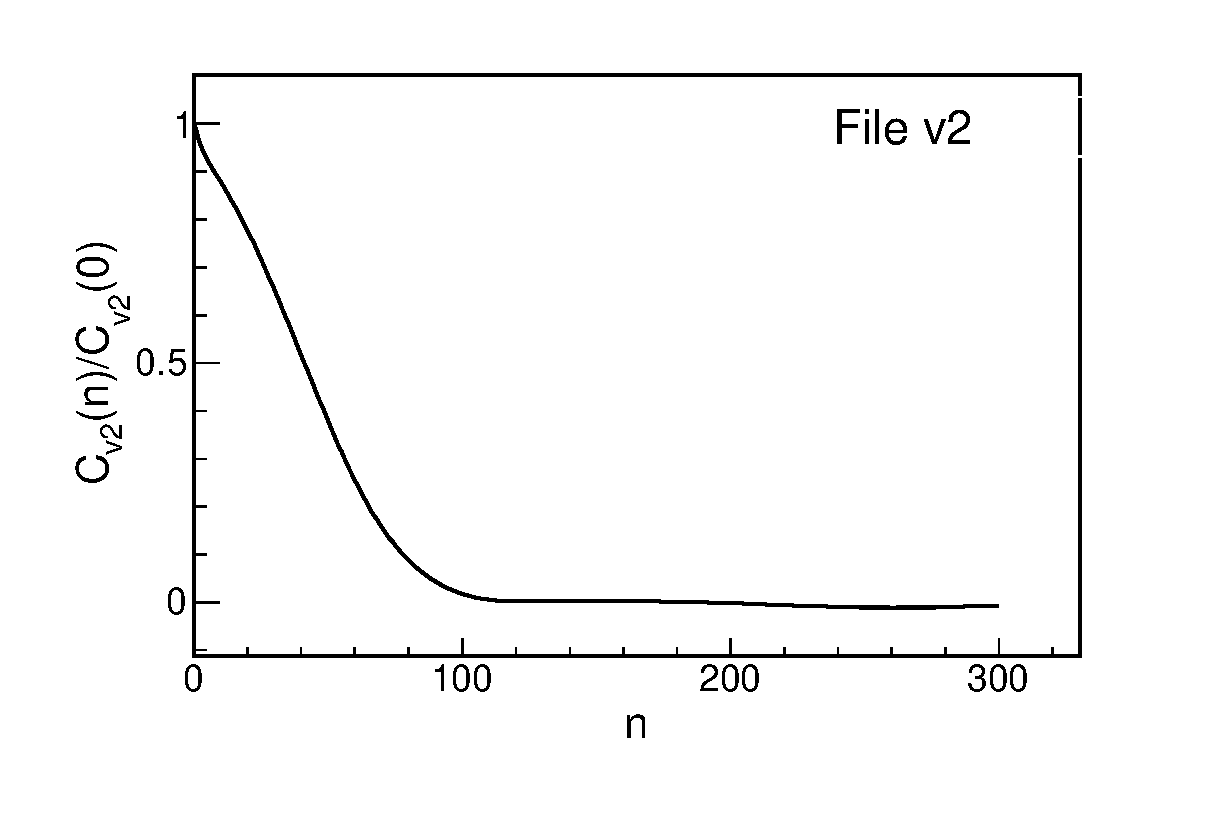
\includegraphics[width=0.5\textwidth]{figures/c2.eps}}\\
  \subfloat[][]{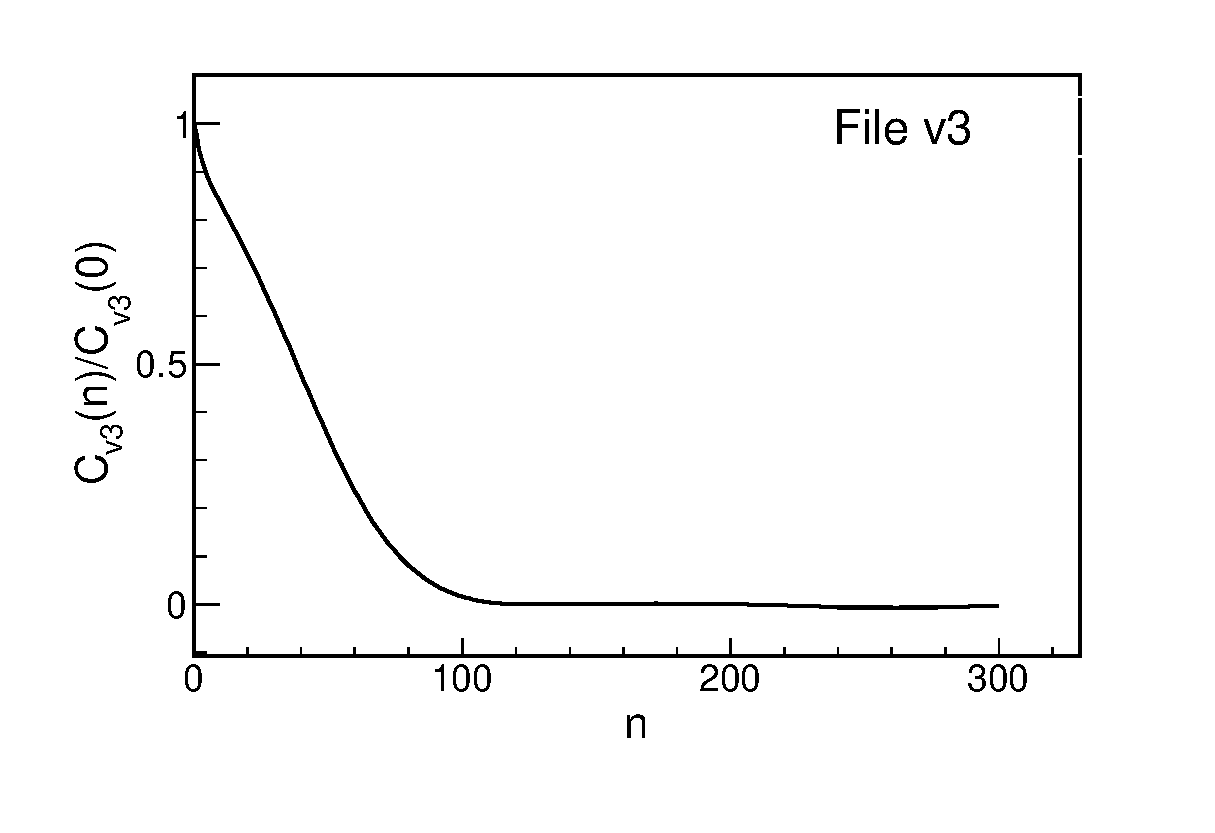
\includegraphics[width=0.5\textwidth]{figures/c3.eps}}
  \subfloat[][]{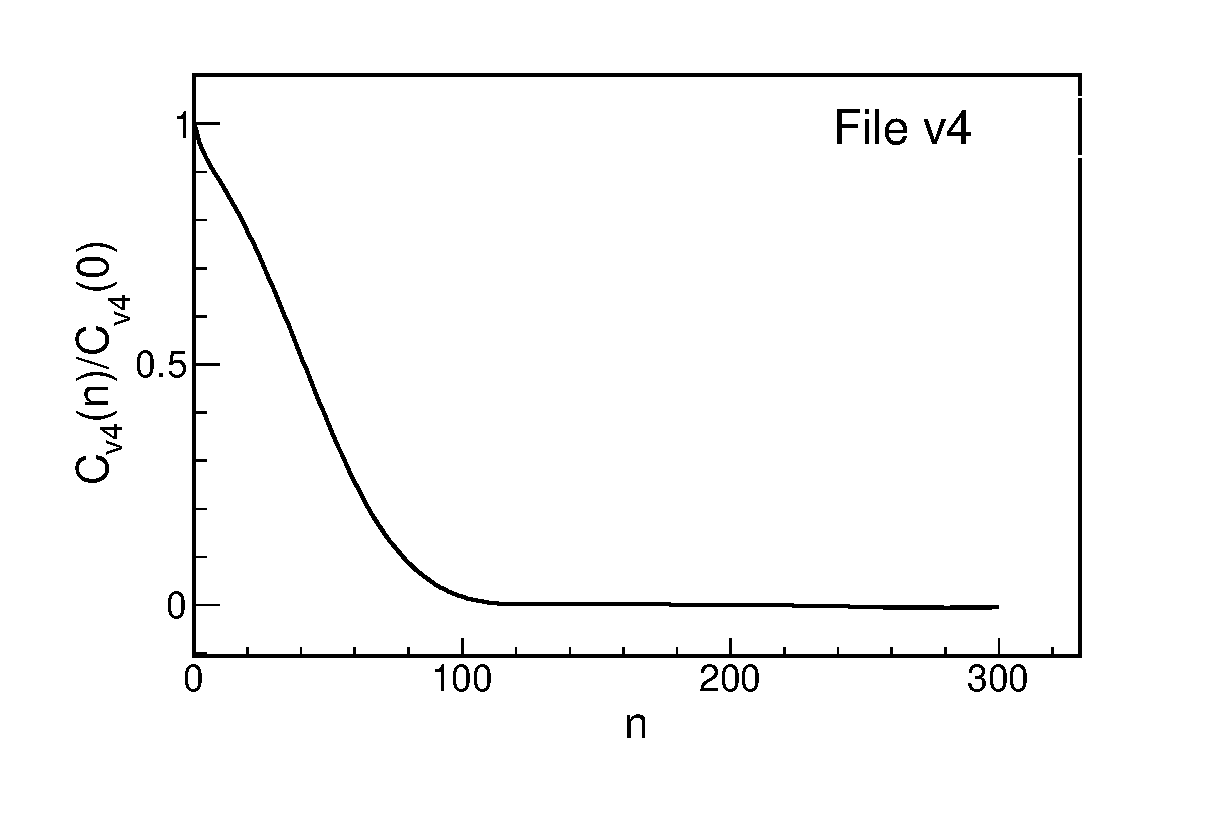
\includegraphics[width=0.5\textwidth]{figures/c4.eps}}\\
  \subfloat[][]{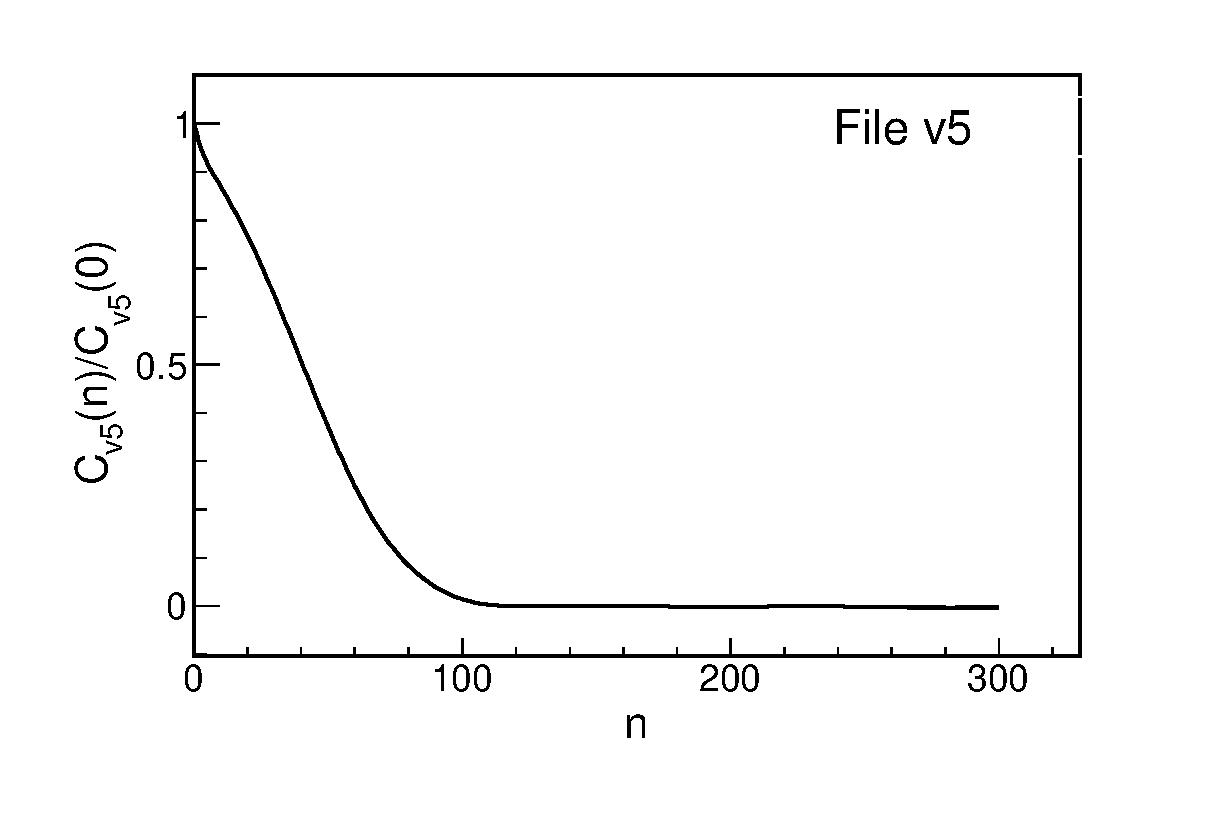
\includegraphics[width=0.5\textwidth]{figures/c5.eps}}
  \caption{\label{corrs} Correlation functions for each of the data sets. It appears each set has auto-correlations on the order of 100 data points.}
\end{figure}
\clearpage
\subsection{4}
We estimate a value of $n_{\text{cut}}=125$. A small deviation in $n_{\text{cut}}$ around this value will not effect the integrated correlation time much. With this value we find the integrated correlation time for each of the data sets as,
\begin{center}
\begin{tabular}{ | c | c | c | c | c |}\hline
  $\tau_{\text{int},\overline{v}_1}$ &  $\tau_{\text{int},\overline{v}_2}$ &  $\tau_{\text{int},\overline{v}_3}$ &  $\tau_{\text{int},\overline{v}_4}$ &  $\tau_{\text{int},\overline{v}_5}$  \\ \hline \hline 
  42.455 & 43.079 & 40.448 & 44.018 & 42.344 \\ \hline
\end{tabular}
\end{center}
\subsection{5}
The true standard deviations of the data are reported in the table below.
\begin{center}
\begin{tabular}{ | c | c | c | c | c |}\hline
  $\hat{\sigma}_{\overline{v}_1}$ &  $\hat{\sigma}_{\overline{v}_2}$ &  $\hat{\sigma}_{\overline{v}_3}$ &  $\hat{\sigma}_{\overline{v}_4}$ &  $\hat{\sigma}_{\overline{v}_5}$  \\ \hline \hline 
  0.8668 & 0.6795 & 0.6377 & 0.6761 & 0.8618 \\ \hline
\end{tabular}
\end{center}
The relation,
\eq{
\hat{\sigma}_{\overline{v}_a,N}=\sqrt{\frac{2\hat{\tau}_{\text{int},\overline{v}_a}}{N}}\hat{\sigma_{v_a}},
}
hold just fine for the data set. Consider the first set $N=1000$,
\eq{
\hat{\sigma}_{\overline{v}_a,N} = (0.866)\l(\sqrt{\frac{2\cdot42.455}{1000}}\r) =  0.252 \approx 0.241.
}
\subsection{6}
The true covarience matrix between the data sets is shown in Fig. \ref{comatrix}.
\begin{figure}[h]
\centering
  \captionsetup[subfigure]{labelformat=empty}
  \subfloat[][]{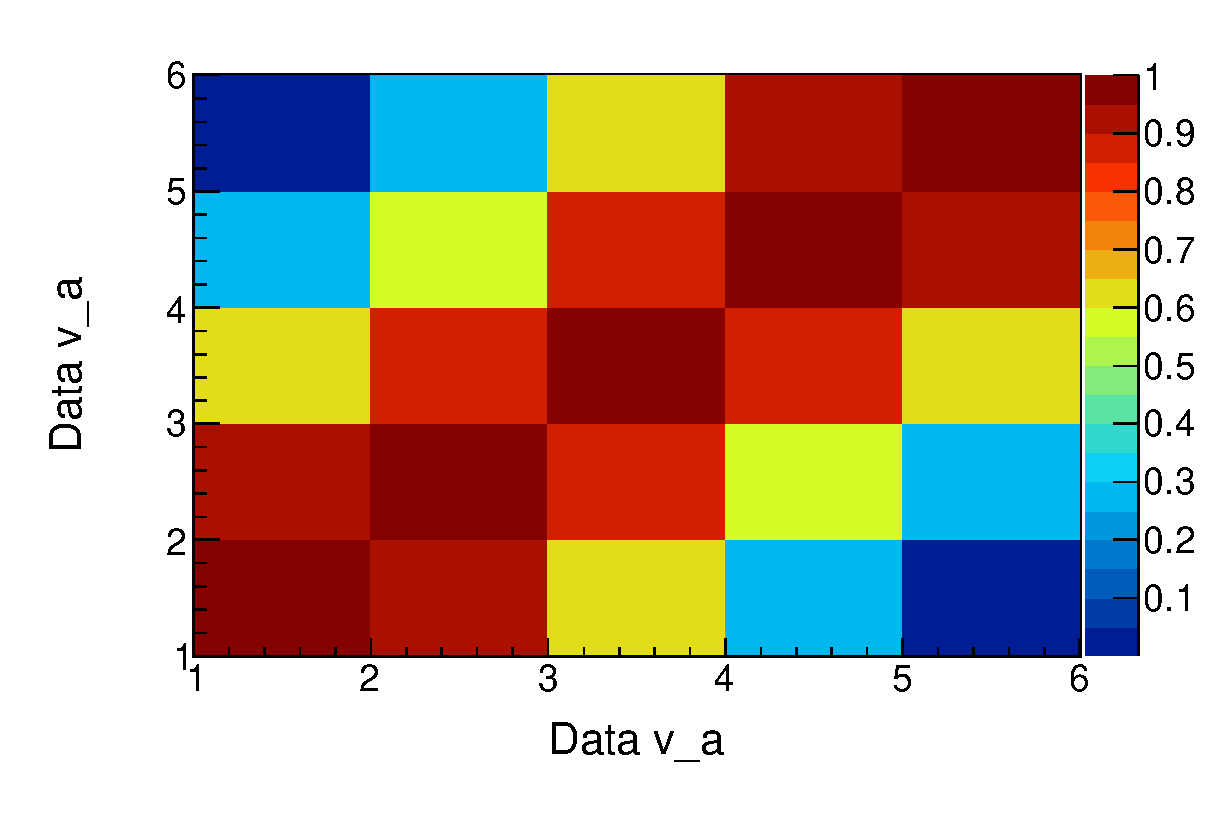
\includegraphics[width=0.5\textwidth]{figures/e1.eps}}
  \subfloat[][]{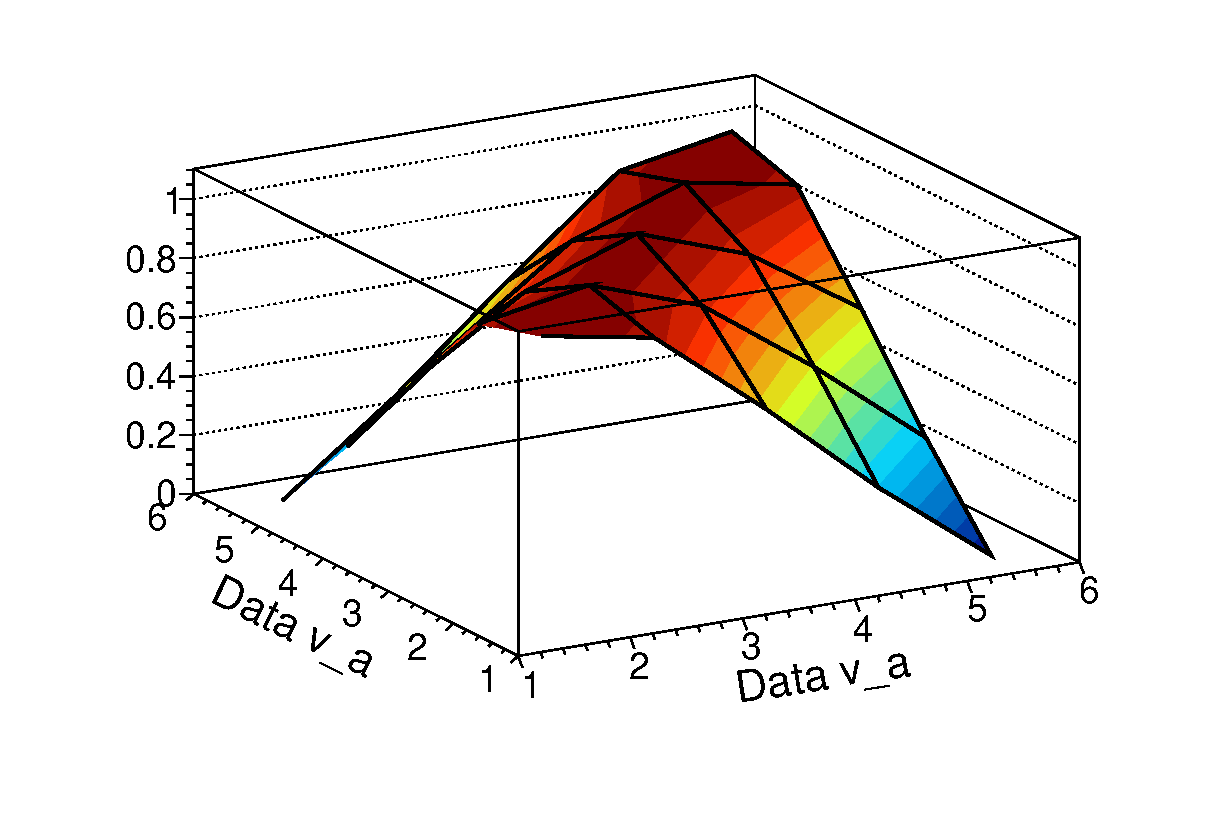
\includegraphics[width=0.5\textwidth]{figures/e2.eps}}\\
\caption{\label{comatrix} Covariance matrix between 5 universe data sets. The left pane is a 2D histogram and in the right plane an equivalent ``surf'' plot generated with ROOT. The Z axis on both plots is the autocorrelation result.}
\end{figure}
\clearpage
\subsection{7}
\begin{center}The code for this problem can be found in \verb|mock_data/mac/secret7.py|. \end{center}
We choose two groups from the full universe of data. One set has $N=1000$ and the other has $N=10000$ representing data from simulation. The autocorrelation function from each of the two groups is plotted in Fig. \ref{ok} for the second data set. Choosing a definite value for $n_{\text{cut}}$ is difficult. We choose $n_{\text{cut}}$ at about 80. The integrated correlation time, standard deviation computed via equation 4 are plotted in the tables below. The two covariance matricies are shown in Fig. \ref{oc}.\\
{\bf N = 1,000}
\begin{center}
\begin{tabular}{ | c | c | c | c | c |}\hline
  $\tau_{\overline{v}_1}$ &  $\tau_{\overline{v}_2}$ &  $\tau_{\overline{v}_3}$ &  $\tau_{\overline{v}_4}$ &  $\tau_{\overline{v}_5}$  \\ \hline \hline 
  42.77605 & 46.42773 & 43.5985 & 39.1126 & 35.12261  \\ \hline
\end{tabular}
\end{center}
\begin{center}
\begin{tabular}{ | c | c | c | c | c |}\hline
  $\hat{\sigma}_{\overline{v}_1}$ &  $\hat{\sigma}_{\overline{v}_2}$ &  $\hat{\sigma}_{\overline{v}_3}$ &  $\hat{\sigma}_{\overline{v}_4}$ &  $\hat{\sigma}_{\overline{v}_5}$  \\ \hline \hline 
  0.24076 & 0.21408 & 0.19337 & 0.16865 & 0.19186 \\ \hline
\end{tabular}
\end{center}
{\bf N = 10,000}
\begin{center}
\begin{tabular}{ | c | c | c | c | c |}\hline
  $\tau_{\overline{v}_1}$ &  $\tau_{\overline{v}_2}$ &  $\tau_{\overline{v}_3}$ &  $\tau_{\overline{v}_4}$ &  $\tau_{\overline{v}_5}$  \\ \hline \hline 
  45.2085 & 47.03129 & 44.13091 & 44.04701 & 41.29598 \\ \hline
\end{tabular}
\end{center}
\begin{center}
\begin{tabular}{ | c | c | c | c | c |}\hline
  $\hat{\sigma}_{\overline{v}_1}$ &  $\hat{\sigma}_{\overline{v}_2}$ &  $\hat{\sigma}_{\overline{v}_3}$ &  $\hat{\sigma}_{\overline{v}_4}$ &  $\hat{\sigma}_{\overline{v}_5}$  \\ \hline \hline 
  0.08663 & 0.06854 & 0.060458 & 0.062144 & 0.076472 \\ \hline
\end{tabular}
\end{center}
Compare these standard deviation values to those seen in the plots of Problem 1 section 2 for each of the data sets. The calculated standard deviations here match those in section 2 {\it closely}!
\begin{figure}[h]
\centering
  \captionsetup[subfigure]{labelformat=empty}
  \subfloat[][]{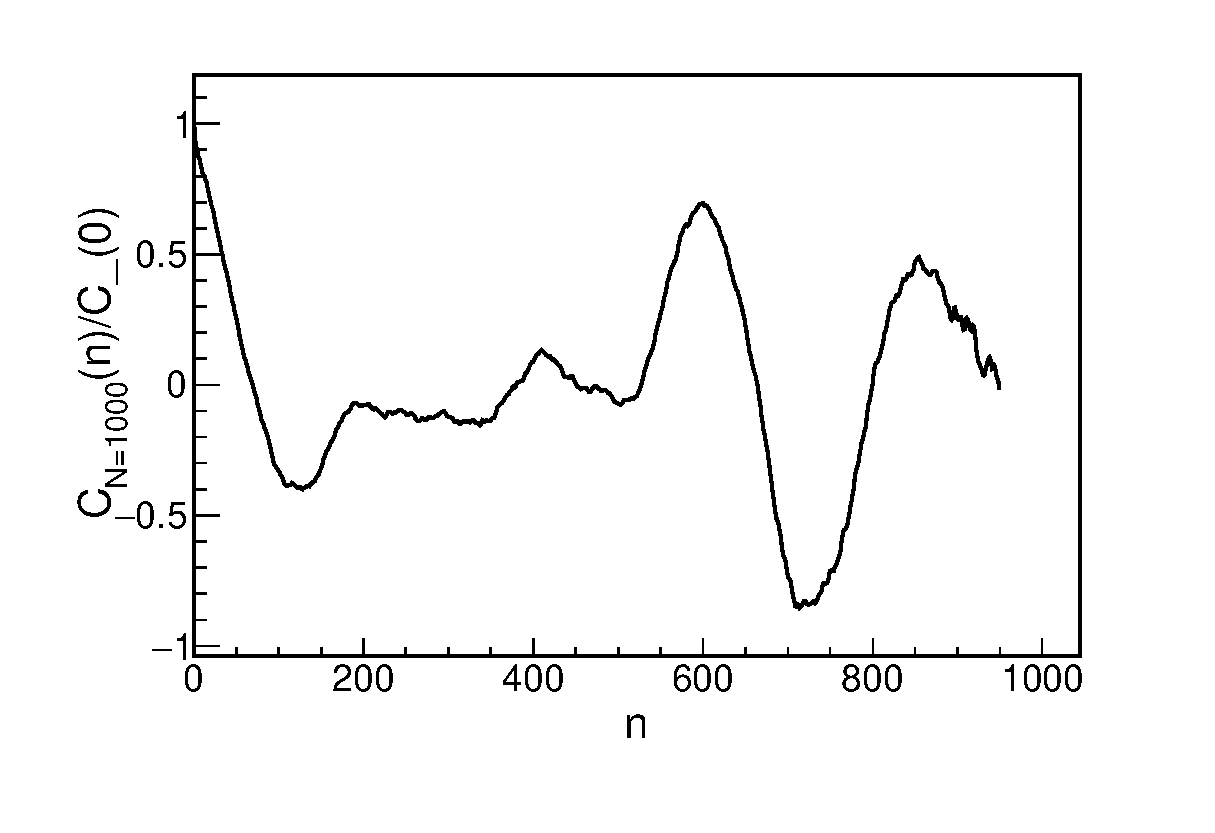
\includegraphics[width=0.5\textwidth]{figures/7one.eps}}
  \subfloat[][]{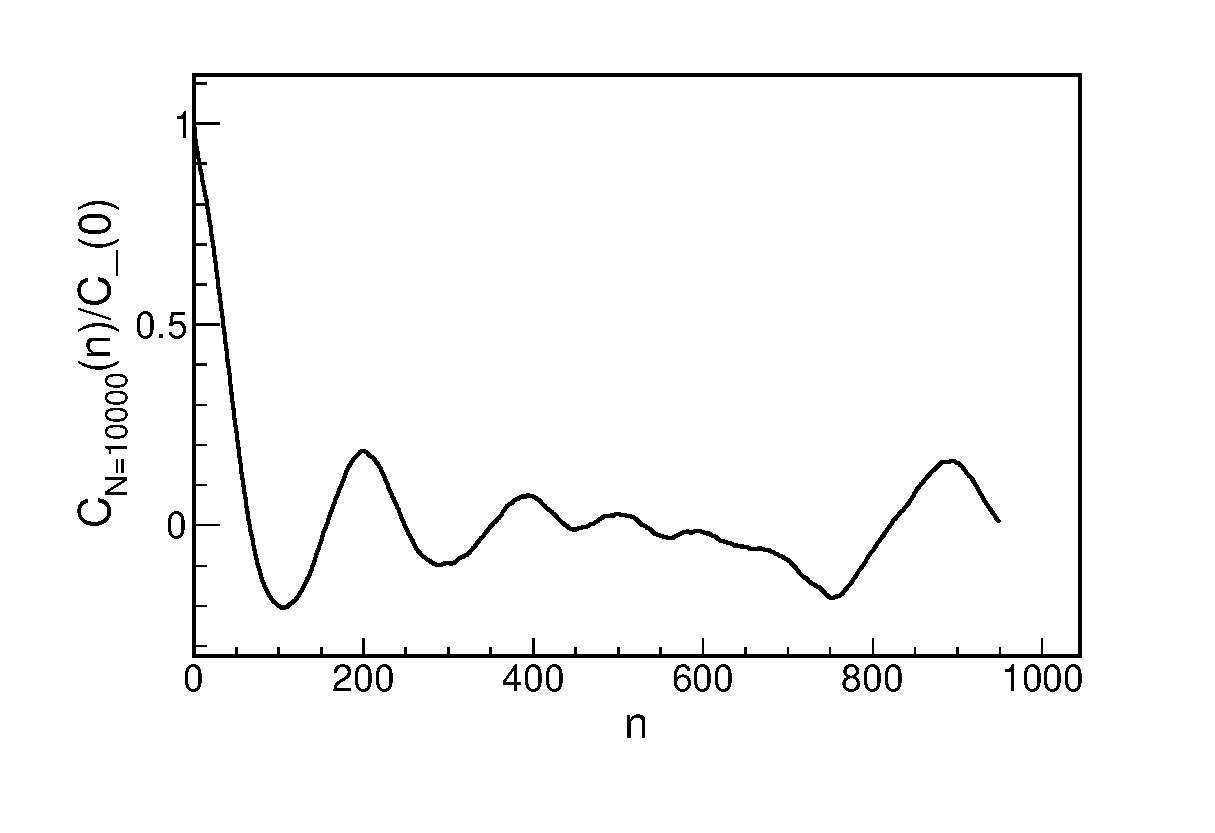
\includegraphics[width=0.5\textwidth]{figures/7two.eps}}\\
\caption{\label{ok} Normalized autocorrelation from two samples of differente sizes in the second data set.}
\end{figure}
\begin{figure}[h]
\centering
  \captionsetup[subfigure]{labelformat=empty}
  \subfloat[][]{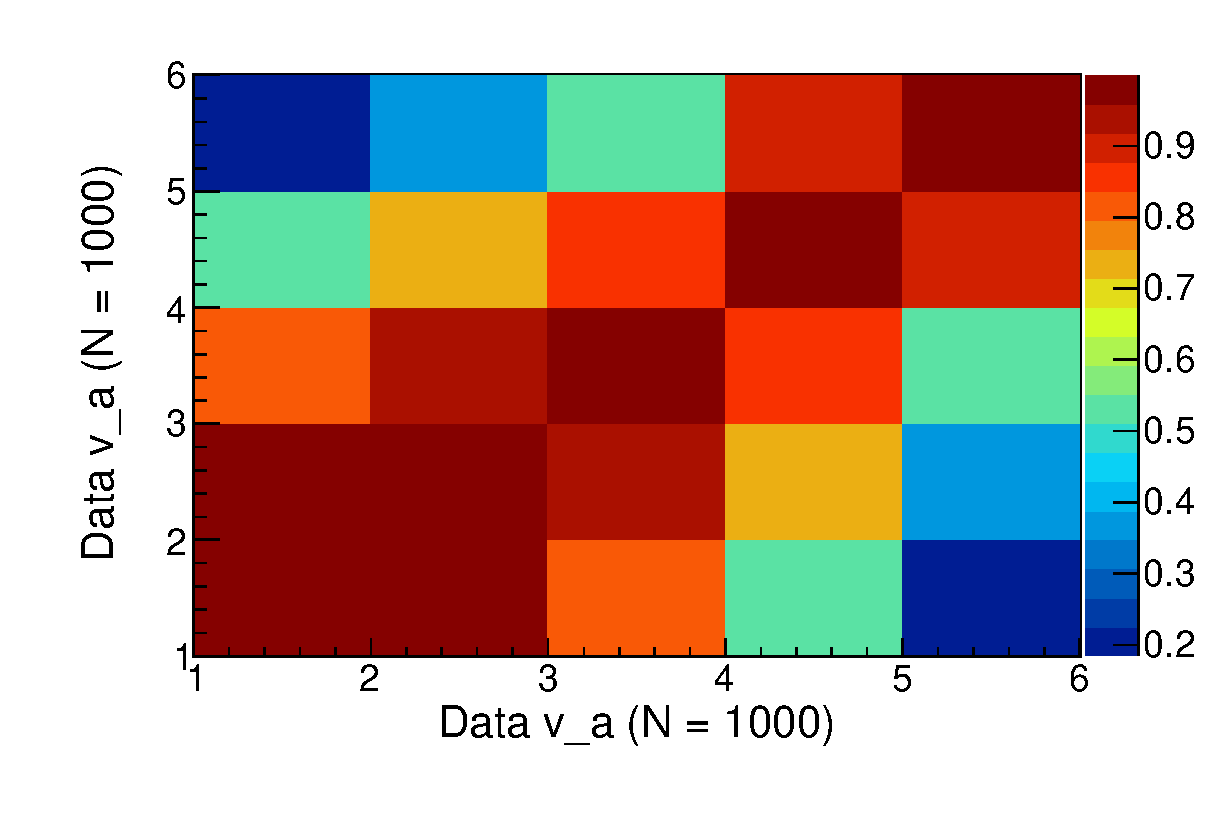
\includegraphics[width=0.5\textwidth]{figures/7corr.eps}}
  \subfloat[][]{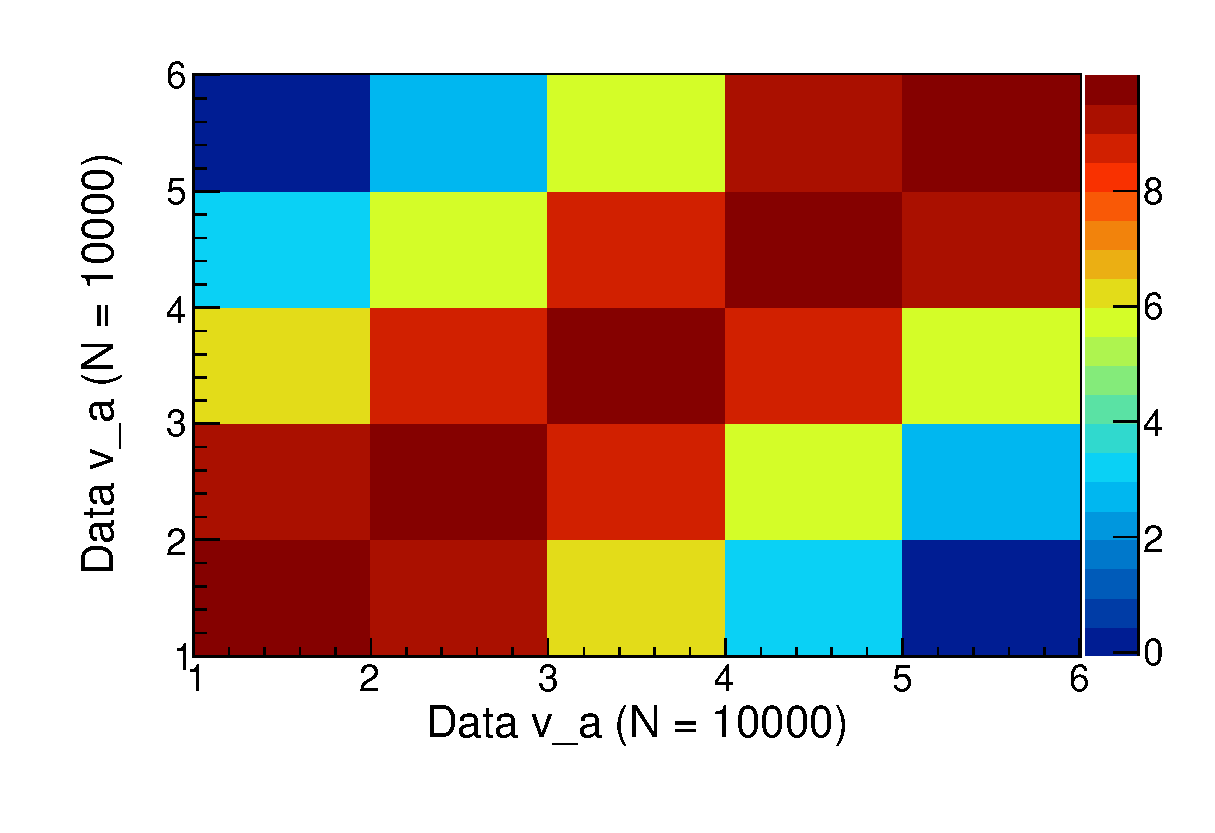
\includegraphics[width=0.5\textwidth]{figures/7corr2.eps}}\\
\caption{\label{ok} Normalized autocorrelation from two samples of differente sizes in the second data set. As N is increased from 1,000 to 10,000, the cross correlation between samples appears to decrease.}
\end{figure}
\clearpage
\section{Problem 2 - Jackknife of Mock Data}
\begin{center}The code for this problem can be found in \verb|mock_data/mac/two.py|. \end{center}
\subsection{1}
We choose sample of size $N=10,000$ for this problem. After breaking up the data into groups, calculating the mean of each, passing they mean through $f_1$, $f_2$, and $f_3$ the following standard deviation are found cross the samples.
\begin{center}
\begin{tabular}{| c | c | c |}
\hline
$\hat{\sigma}_{f_1,N}$ & $\hat{\sigma}_{f_2,N}$ & $\hat{\sigma}_{f_3,N}$ \\ \hline\hline
0.016074 & 0.009445 & 0.037722 \\ \hline 
\end{tabular}
\end{center}

\subsection{2}
Calculation of standard deviation from native propagation of errors is as follows.
$\mathbf{f_1}$
\eq{
\sigma_{f_1}^2 &= \l(\frac{\partial f_1}{\partial \overline{v}_1}\r)^2\sigma_{\overline{v}_1}^2 + \l(\frac{\partial f_1}{\partial \overline{v}_2}\r)^2\sigma_{\overline{v}_2}^2,\\
&=\l(\frac{1}{\overline{v}_2}\r)^2\sigma_{\overline{v}_1}^2 + \l(\frac{\overline{v}_1}{\overline{v}_2^2}\r)^2\sigma_{\overline{v}_2}^2,
}
so
\eq{
\boxed{\sigma_{f_1}=\sqrt{\l(\frac{1}{\overline{v}_2}\r)^2\sigma_{\overline{v}_1}^2 + \l(\frac{\overline{v}_1}{\overline{v}_2^2}\r)^2\sigma_{\overline{v}_2}^2}.}
}
$\mathbf{f_2}$
\eq{\sigma_{f_2}^2 &= \l(\frac{\partial f_2}{\partial \overline{v}_3}\r)^2\sigma_{\overline{v}_3}^2 + \l(\frac{\partial f_2}{\partial \overline{v}_4}\r)^2\sigma_{\overline{v}_4}^2,\\ 
  &=\exp\l(2(\overline{v}_3-\overline{v}_4)\r)\l(\sigma_{\overline{v}_3}^2+\sigma_{\overline{v}_4}^2\r),
}
so
\eq{
\boxed{ \sigma_{f_2} = \exp\l(\overline{v}_3-\overline{v}_4\r)\sqrt{\sigma_{\overline{v}_3}^2+\sigma_{\overline{v}_4}^2}}.
}
$\mathbf{f_3}$
\eq{
\sigma_{f_3}^2 &= \l(\frac{\partial f_3}{\partial \overline{v}_1}\r)^2\sigma_{\overline{v}_1}^2 + \l(\frac{\partial f_3}{\partial \overline{v}_2}\r)^2\sigma_{\overline{v}_2}^2 + \l(\frac{\partial f_3}{\partial \overline{v}_3}\r)^2\sigma_{\overline{v}_3}^2 + \l(\frac{\partial f_3}{\partial \overline{v}_4}\r)^2\sigma_{\overline{v}_4}^2 + \l(\frac{\partial f_3}{\partial \overline{v}_5}\r)^2\sigma_{\overline{v}_5}^2,
}
so
\eq{
\boxed{\sigma_{f_3} = \sqrt{\log^2(\overline{v}_5) \left(\frac{\overline{v}_1^2 \sigma_{\overline{v}_2}^2}{\overline{v}_2^4}+\frac{\sigma_{\overline{v}_1}^2}{\overline{v}_2^2}+\frac{\overline{v}_3^2 \sigma_{\overline{v}_4}^2}{\overline{v}_4^4}+\frac{\sigma_{\overline{v}_3}^2}{\overline{v}_4^2}\right)+\frac{\sigma_{\overline{v}_5}^2 (\overline{v}_1 \overline{v}_4+\overline{v}_2 \overline{v}_3)^2}{\overline{v}_2^2\,\overline{v}_4^2\,\overline{v}_5^2}}}
}
Applying these formulas to the sample means and the sample mean standard deviation gives the following values (assuming no autocorrelation):
\begin{center}
\begin{tabular}{| c | c | c |}
\hline
$\hat{\sigma}_{f_1,N}$ & $\hat{\sigma}_{f_2,N}$ & $\hat{\sigma}_{f_3,N}$ \\\hline\hline
0.031368 & 0.026419 & 0.065233 \\ \hline
\end{tabular}
\end{center}
The values from native propagation of errors do not resemble those of the true standard deviations calculated in the previous section.
\subsection{3}
With the jackknife procedure implemented in \verb|two.py| we plot the the standard deviation of the jacknife values versus the bin size and find that the standard deviation levels off a precisely the autocorrelation time found in the first problem (roughly 125). In this section we use a sample of $N=10,000$. The results can be found in Fig. \ref{jacks}. Choosing a bin size of 125 (a total of 80 bins) yields the following values for the jackknife means and standard deviations side by side with the true sample wise mean and standard deviations. The values are {\it very} similar.
\begin{center}
\begin{tabular}{| c | c | c | c | c | c |} \hline
$\hspace{2pt} & $\overline{v}_1$ & $\overline{v}_2$ & $\overline{v}_3$ & $\overline{v}_4$ & $\overline{v}_5$\\ \hline \hline
True mean & 1.76084 & 2.88634 & 4.01185 & 5.13712 & 6.26238\\ \hline
Jack mean & 1.74052 & 2.85721 & 3.97391 & 5.11390 & 6.25388\\ \hline 
\end{tabular}
\end{center}

\begin{center}
\begin{tabular}{| c | c | c | c | c | c |} \hline
$\hspace{2pt} & $\hat{\sigma}_{v_1}$ & $\hat{\sigma}_{v_2}$ & $\hat{\sigma}_{v_3}$ & $\hat{\sigma}_{v_4}$ & $\hat{\sigma}_{v_5}$\\ \hline \hline
True std & 0.08172 & 0.06867 & 0.05606 & 0.05901 & 0.07424\\ \hline
Jack std & 0.07263 & 0.05517 & 0.04884 & 0.05656 & 0.07462\\ \hline
\end{tabular}
\end{center}
\begin{figure}[h]
\centering
  \captionsetup[subfigure]{labelformat=empty}
  \subfloat[][]{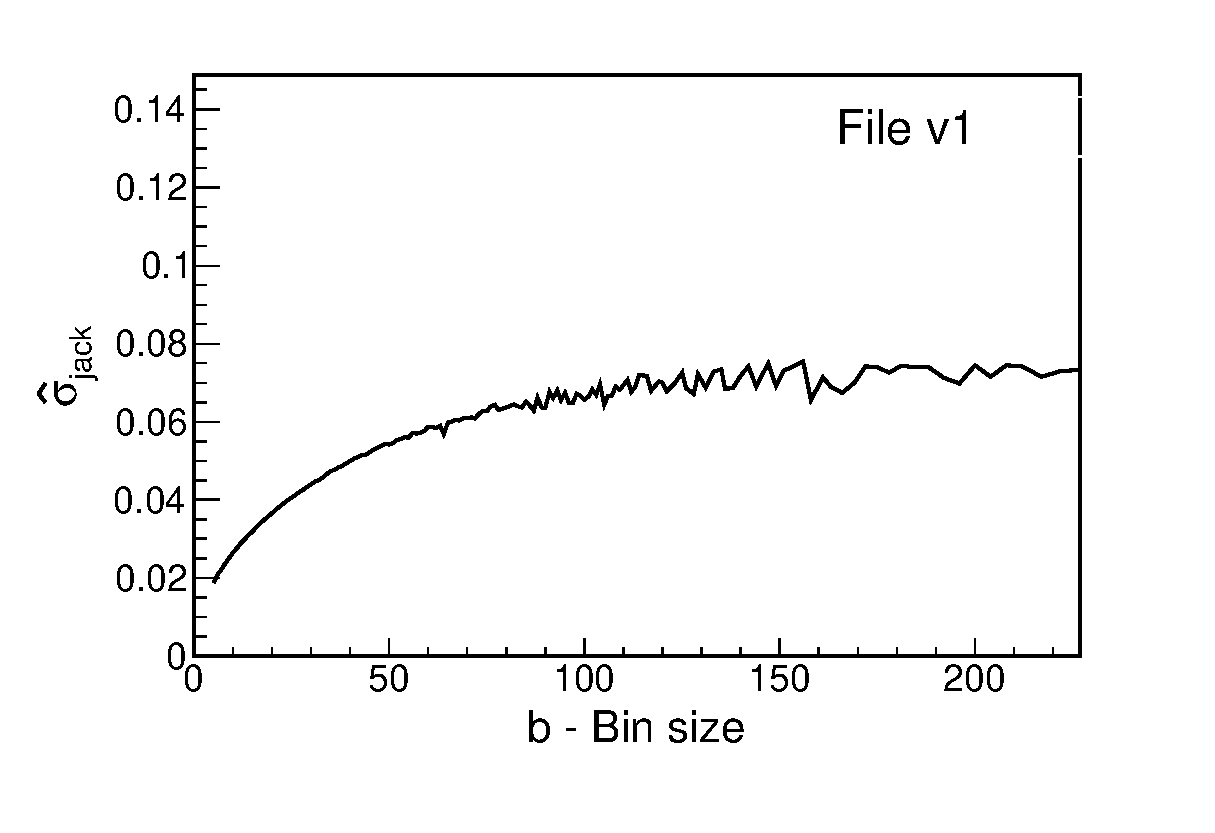
\includegraphics[width=0.5\textwidth]{figures/v1jack.eps}}
  \subfloat[][]{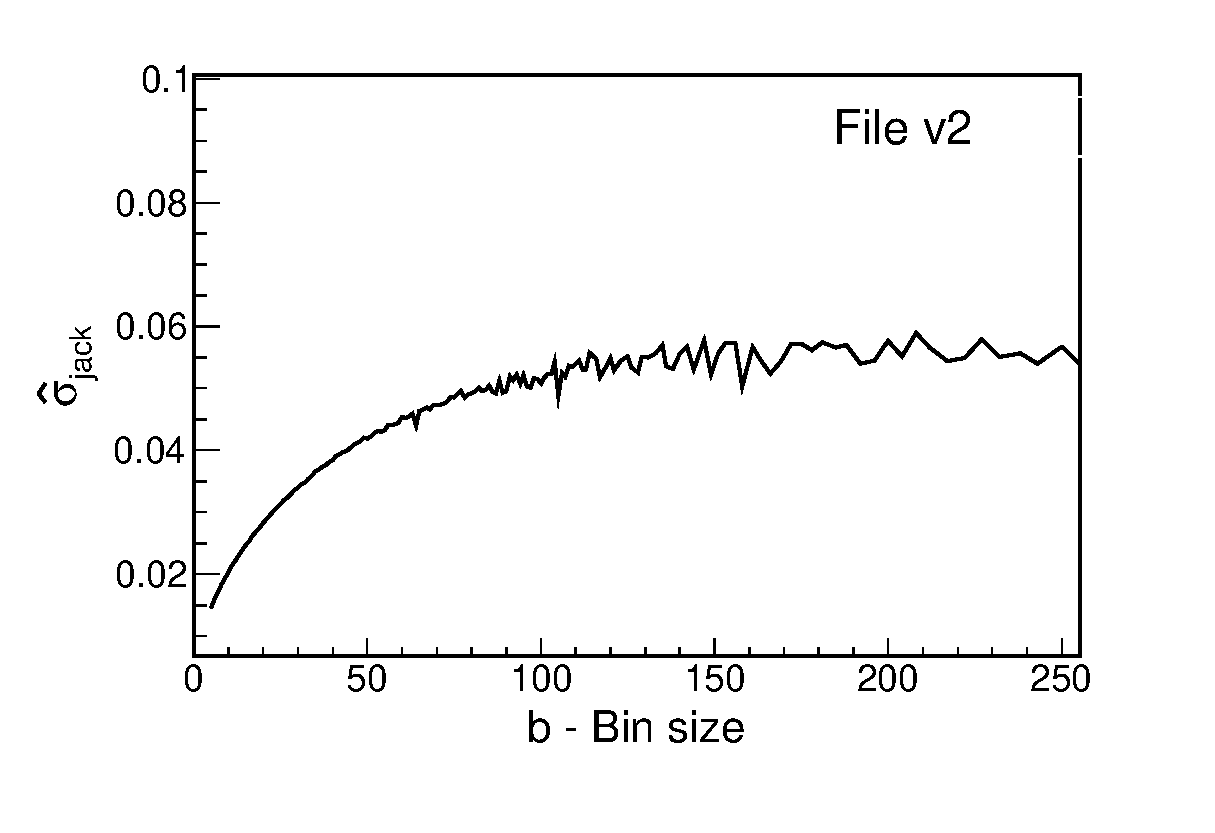
\includegraphics[width=0.5\textwidth]{figures/v2jack.eps}}\\
  \subfloat[][]{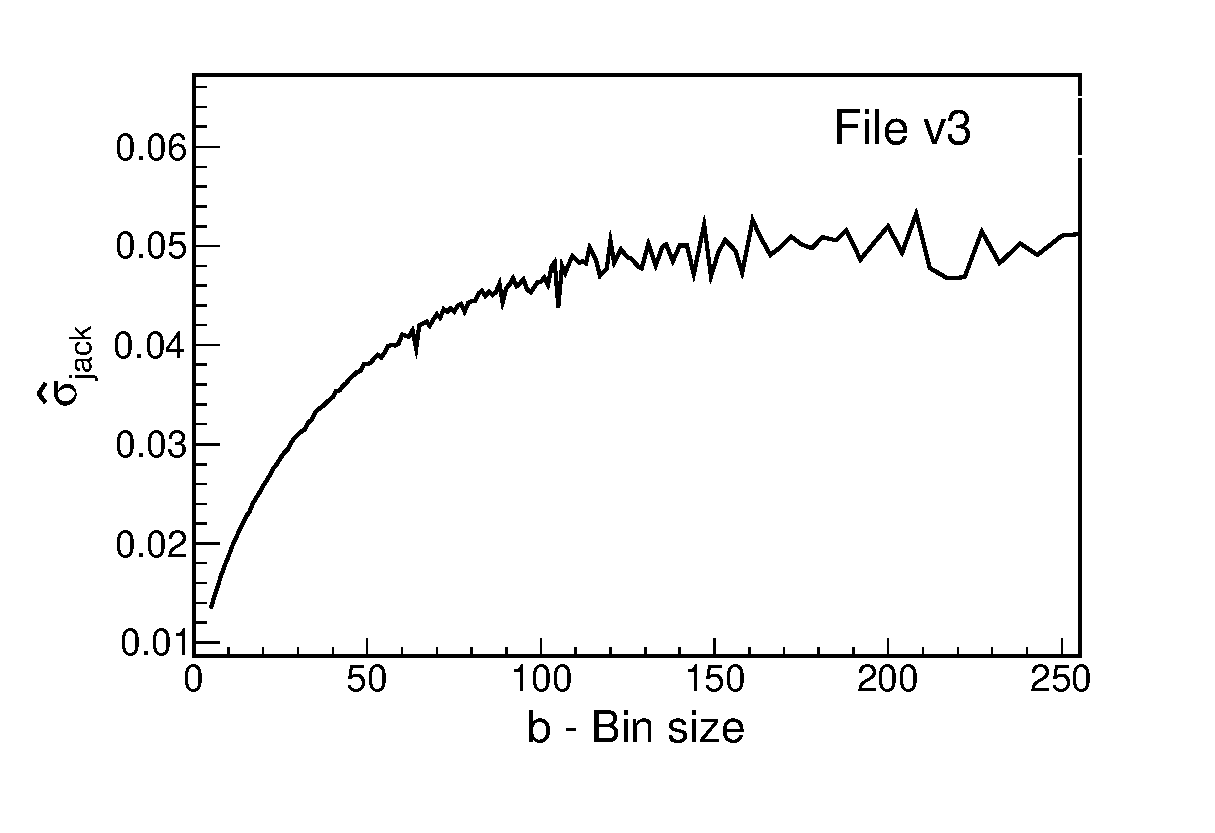
\includegraphics[width=0.5\textwidth]{figures/v3jack.eps}}
  \subfloat[][]{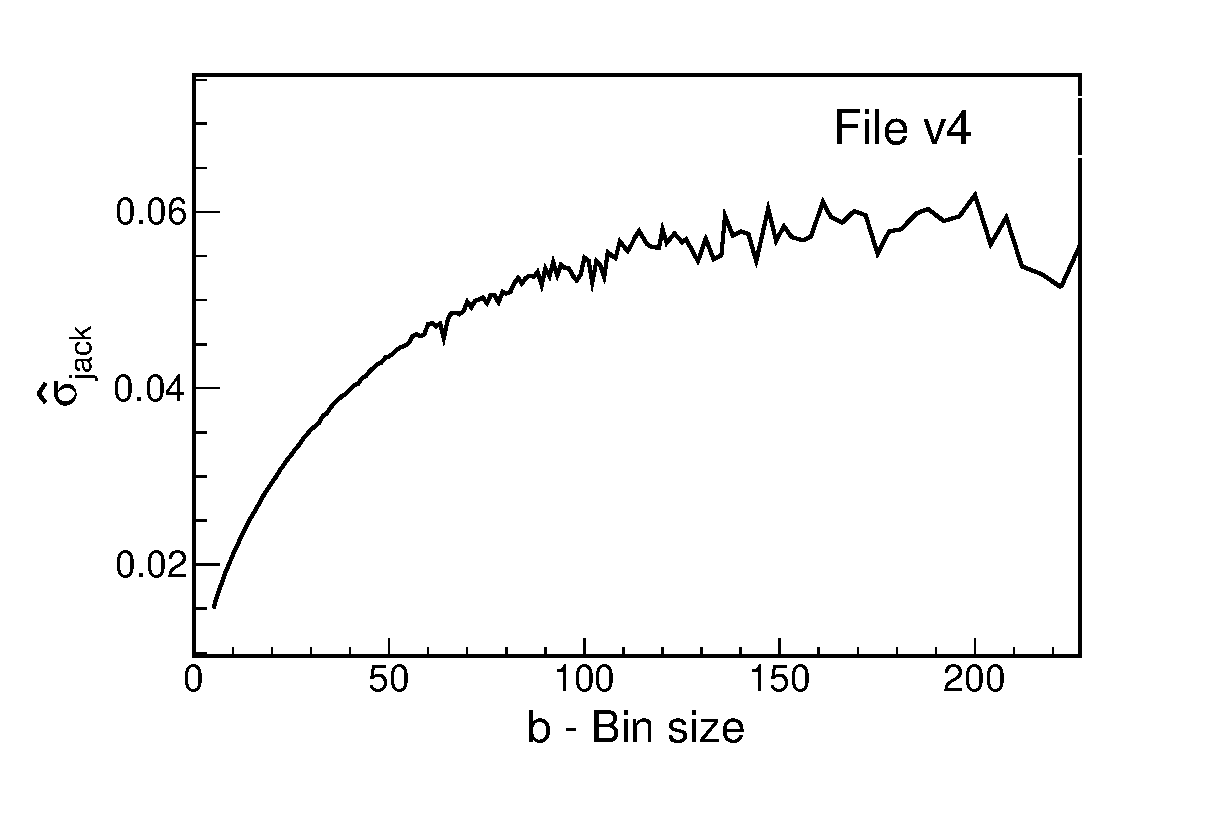
\includegraphics[width=0.5\textwidth]{figures/v4jack.eps}}\\
  \subfloat[][]{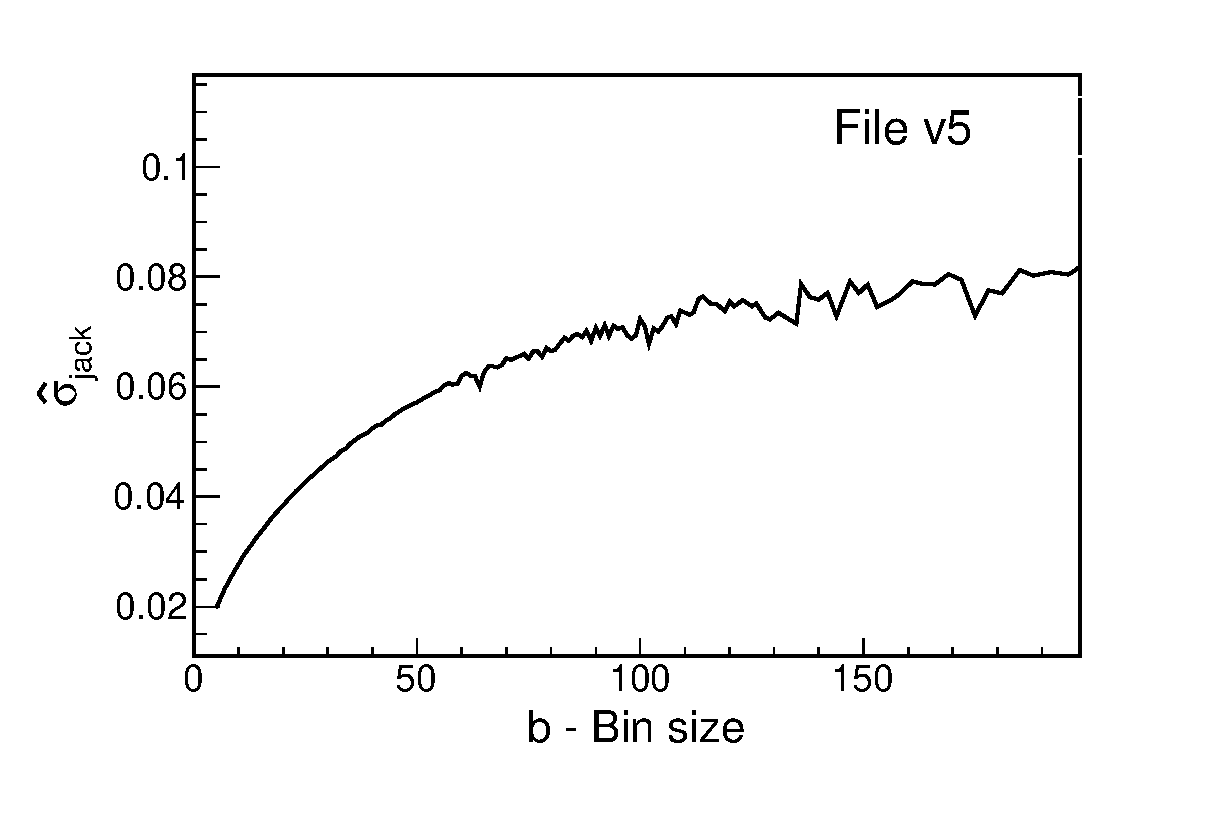
\includegraphics[width=0.5\textwidth]{figures/v5jack.eps}}
\caption{\label{jacks} Jacknife standard deviation for five data sets showing expected ``leveling off'' at the autocorrelation time.}
\end{figure}
 The jackknife seems successful
\subsection{4}
We calculate the error on the three functions for each of the $N/b$ jackknife blocks and determine their associated errors given by equation 11. The results are as follows.
\begin{center}
\begin{tabular}{| c | c | c |}
\hline
$\hat{\sigma}_{f_1,N,\text{jack}}$ & $\hat{\sigma}_{f_2,N,\text{jack}}$ & $\hat{\sigma}_{f_3,N,\text{jack}}$ \\ \hline\hline
0.014929 & 0.00892 & 0.03346 \\ \hline 
\end{tabular}
\end{center}
The values are nearly identical to the true errors on the functions found in the first section! The jackknife appears successful!!!
\clearpage
\section{Problem 3 - Autocorrelation Time Estimator}
\begin{center}The code for this problem can be found in \verb|mock_data/mac/three.py|, and in \verb|mock_data/src/Analyzer.*| \end{center}
We investigate the error on $\tau_{\text{int}}$ We choose two values for $N$ (1000 and 10000) and calculate the standard deviation of the integrated correlation time and plot it as a function of $n_{\text{cut}}$ as shown in Fig. \ref{three}. An obvious divergence is observed in the $N=1000$ sample as $n_{\text{cut}}$ is varied up to 1000. The standard deviation of $\tau$ {\bf increased slower} for the $N=10000$ data set than the $N=1000$ as $n_{\text{cut}}$ is increased. The standard deviation is {\bf larger} for the $N=1000$ data set.
\begin{figure}[h]
\centering
  \captionsetup[subfigure]{labelformat=empty}
  \subfloat[][]{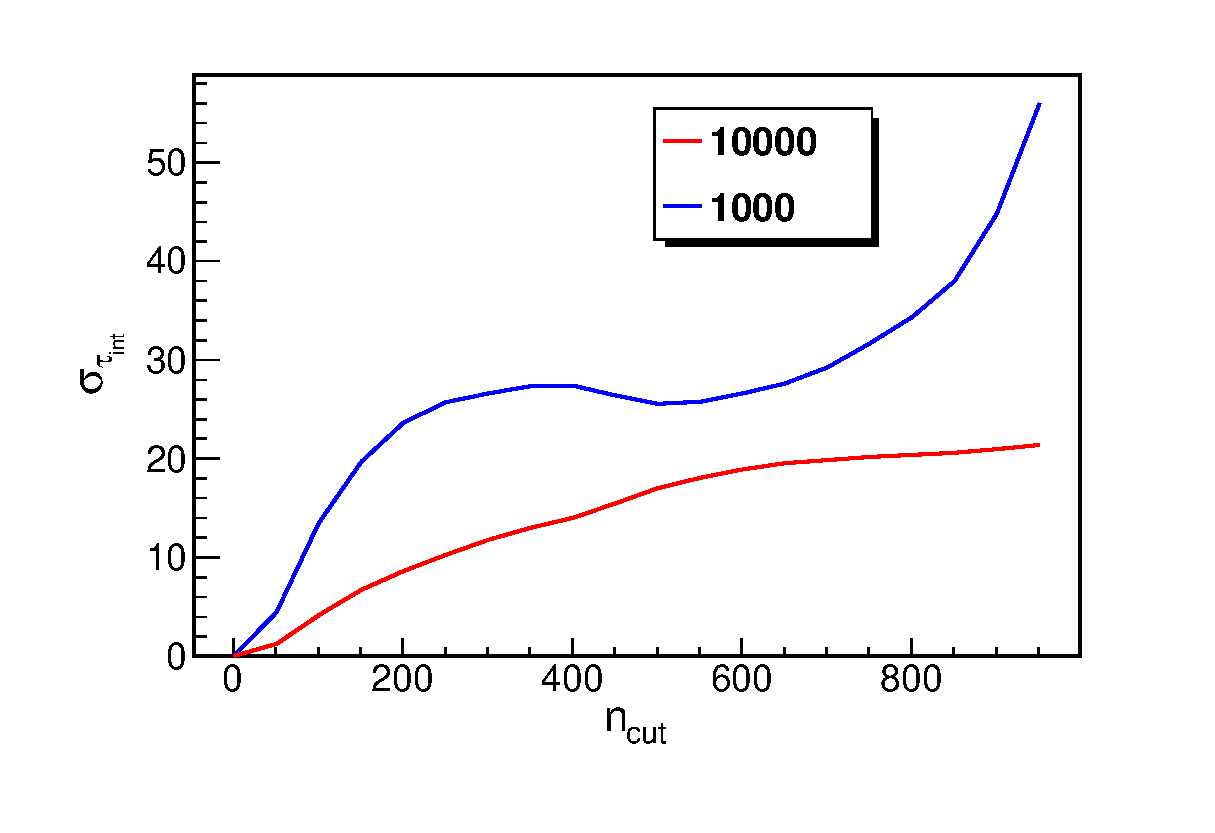
\includegraphics[width=0.5\textwidth]{figures/num_3.eps}}
\caption{\label{three} Standard deviation of the integrated correlation time versus the $n_{\text{cut}}$ variable. Divergence is observed in both sample sizes.}
\end{figure}
\clearpage
\section{Problem 4 - LArgon Stats}
We have evolved the Liquid argon simulation with $1000$ particles over 5000 steps with a density of 1.0. The plots for autocorrelation in the potential energy, temperature, and the virial are shown in Fig. \ref{lauto}. From inspection of the autocorrelation plots, a suitable value of $n_{\text{cut}}$ should be approximately {\bf 200}. The correlation matrix for the three variables is shown in Fig. \ref{larcorr}. The potential energy and virial variables are completely correlated as they are both derived from the same function. On the other hand the temperature is completely anti-correlated as expected due to conservation of total energy. The temperature is derived from the kinetic energy which is contrained by the potential, hence the variables are anti-correlated. 
\begin{figure}[h]
\centering
  \captionsetup[subfigure]{labelformat=empty}
  \subfloat[][]{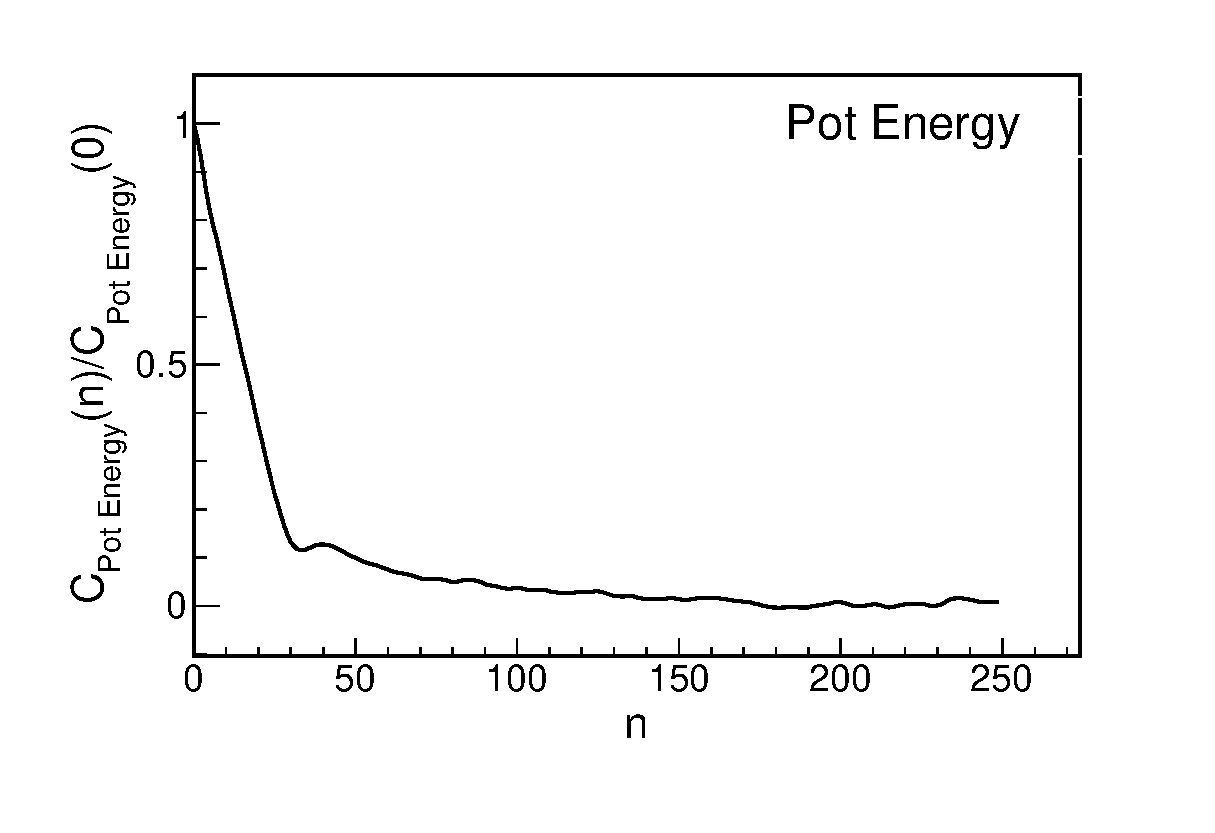
\includegraphics[width=0.5\textwidth]{figures/4PE_corr.eps}}
  \subfloat[][]{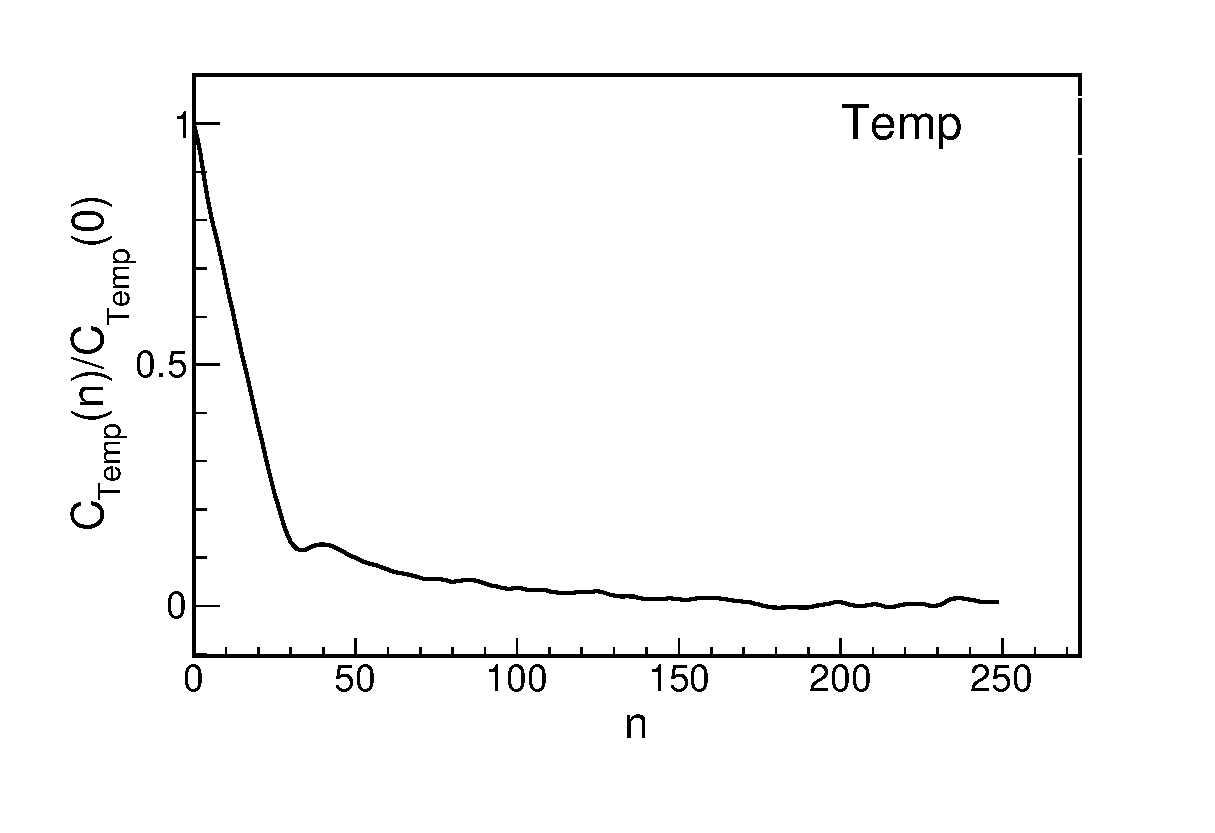
\includegraphics[width=0.5\textwidth]{figures/4T_corr.eps}}\\
\subfloat[][]{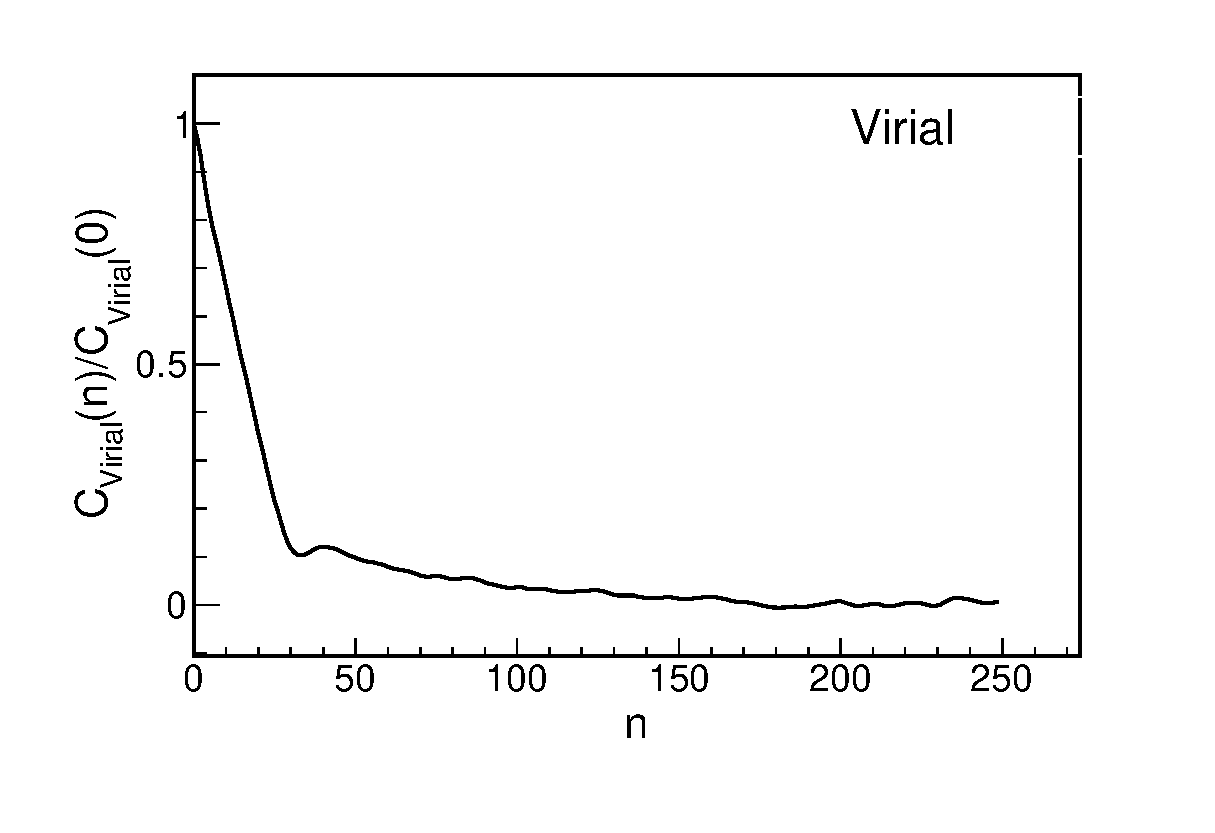
\includegraphics[width=0.5\textwidth]{figures/4Vir_corr.eps}} 
\caption{\label{lauto} Liquid argon normalized autocorrelation time for potential energy, temperature, and the virial.}
\end{figure}
\begin{figure}[h]
\centering
  \captionsetup[subfigure]{labelformat=empty}
  \subfloat[][]{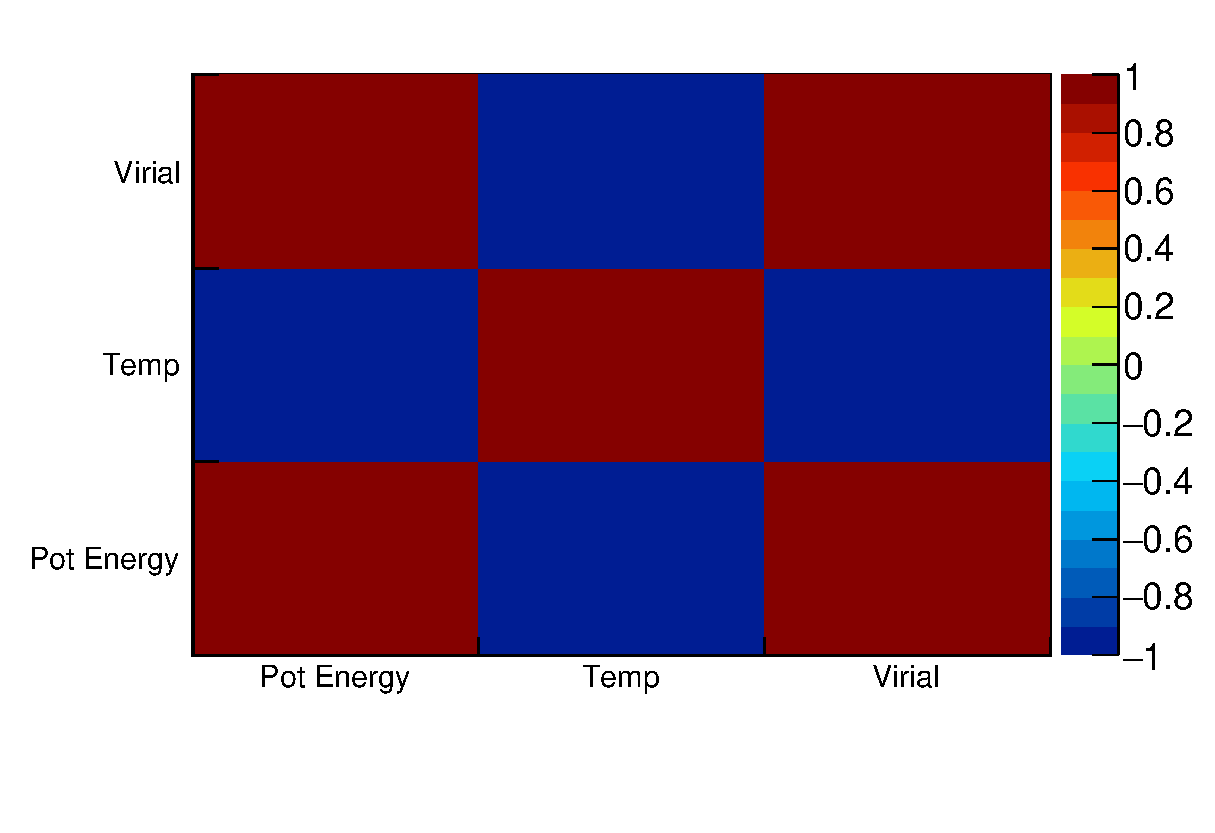
\includegraphics[width=0.5\textwidth]{figures/covariance.eps}}
\caption{\label{larcorr} Correlation matrix for potential energy, temperature, and virial. }
\end{figure}


\end{document}
